\chapter{3D Vision}

\section{Image Formation}

The basic model is based on the principle of \textbf{camera obscura}, a room with a hole by which the light can enter the room.

\begin{figure}[H]
    \centering
    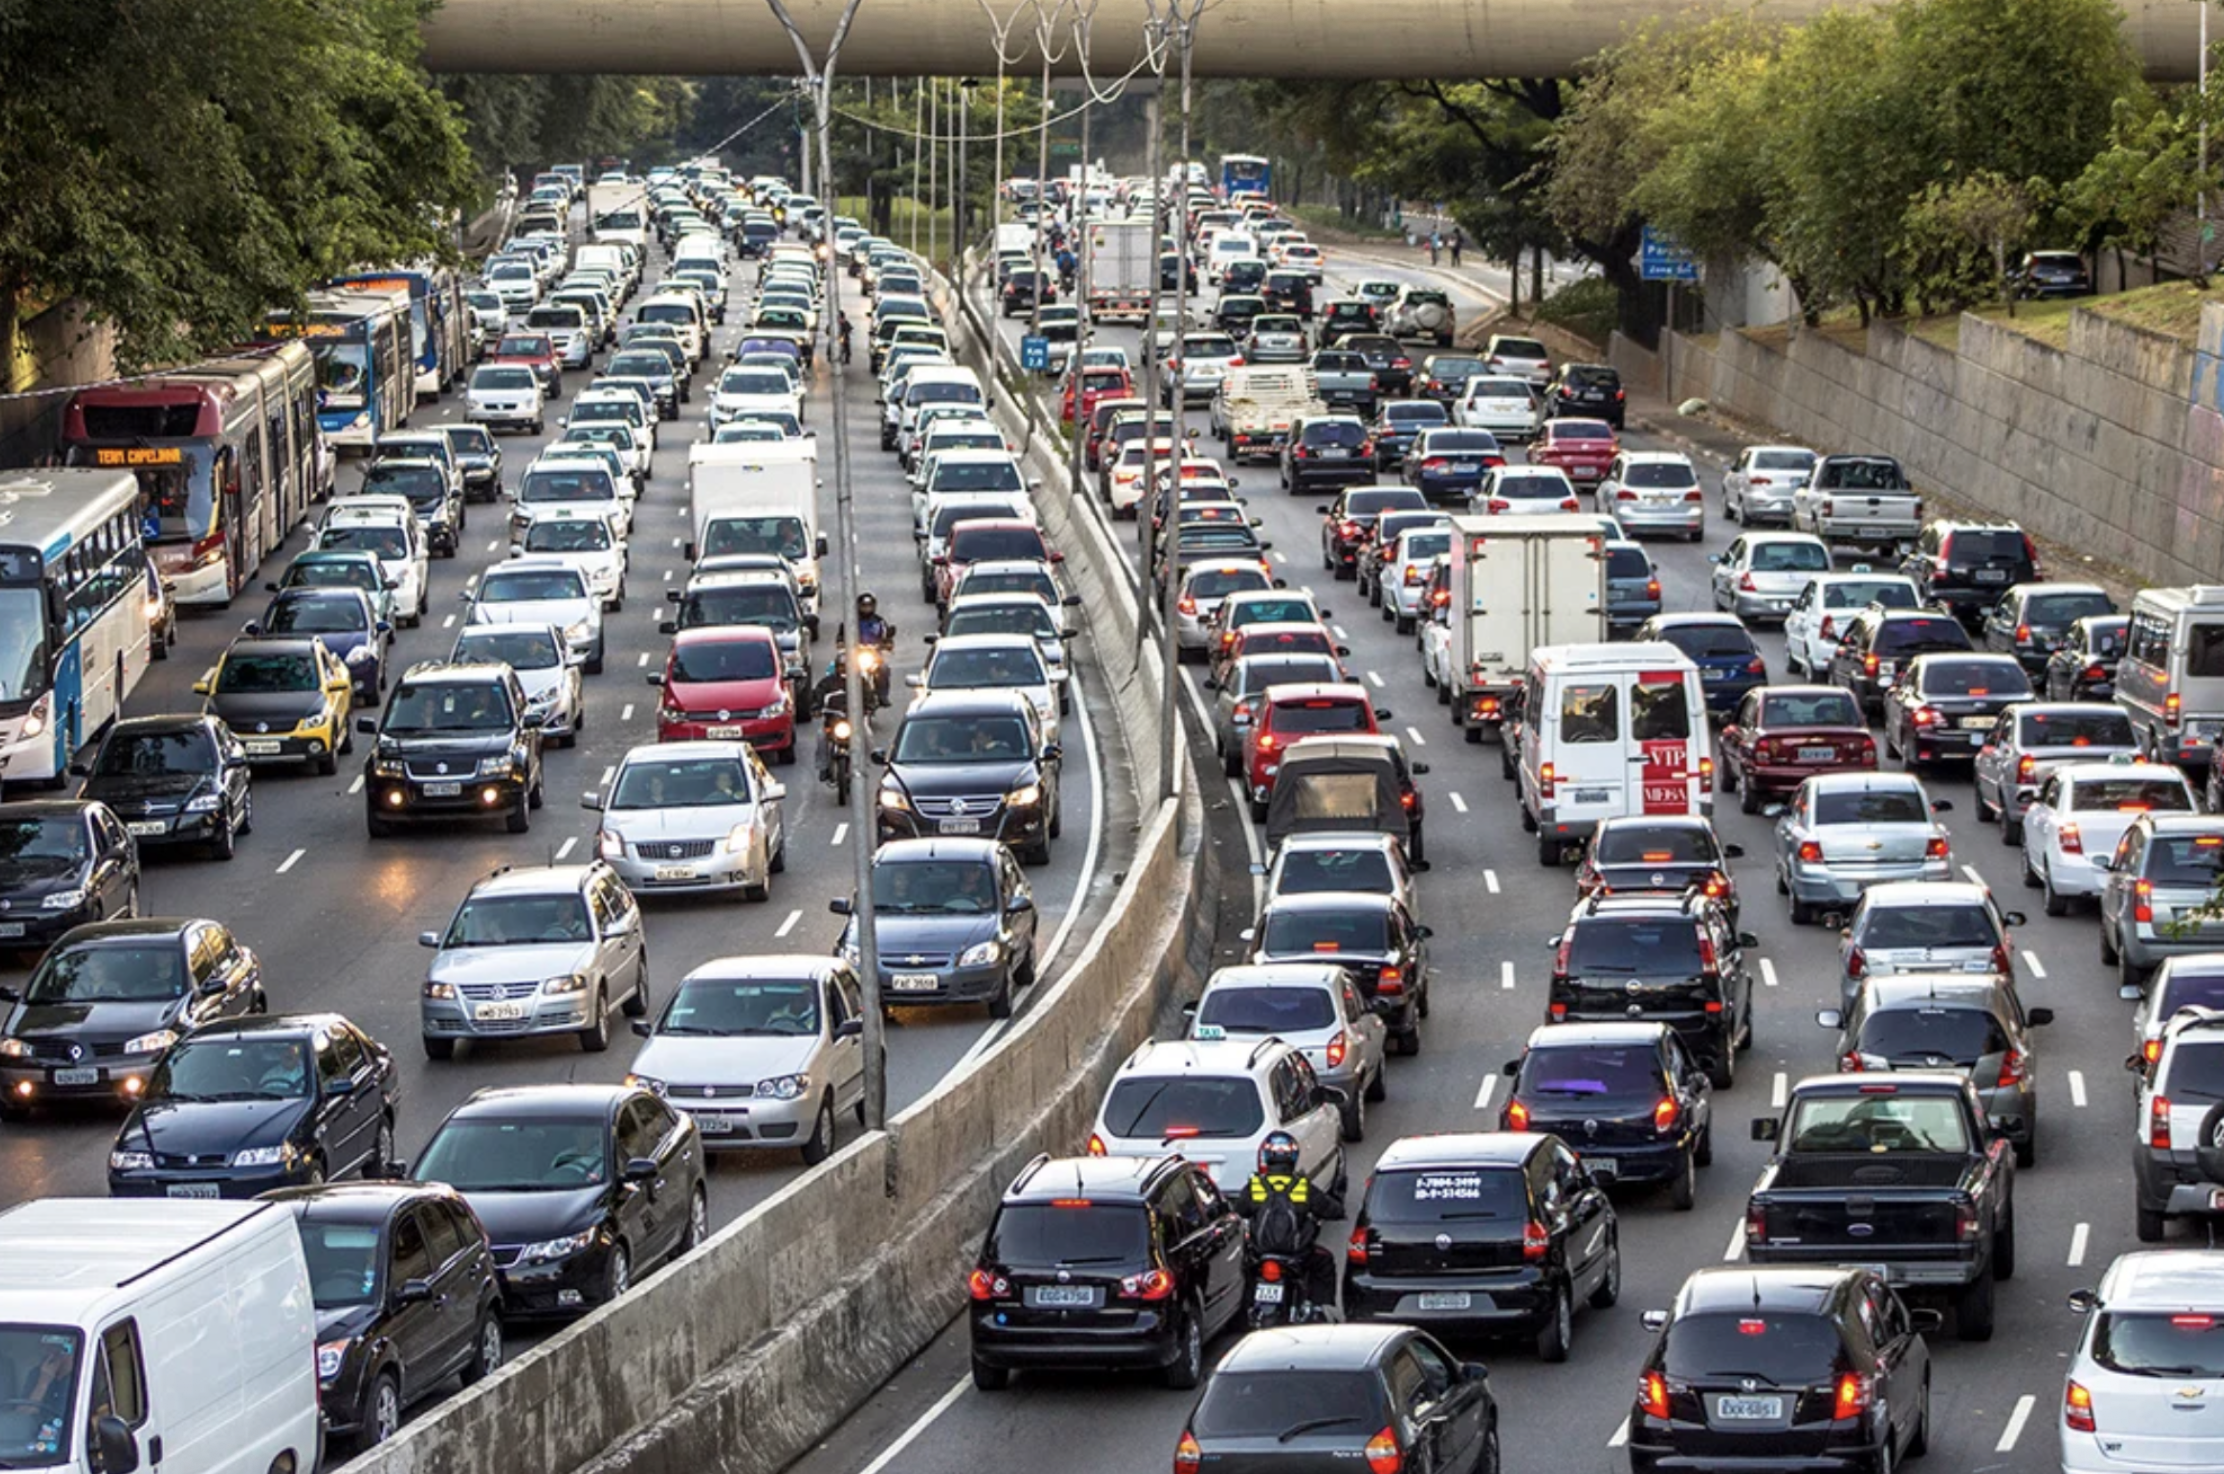
\includegraphics[width=0.6\textwidth]{assets/ch2/1.png}
    \caption{Camera Obscura principle.}
    \label{fig:camera_obscura}
\end{figure}

A simple setting for creating images on a white piece of paper is by projecting a shadow on it and, in the middle of the shadow, appears a picture of the scene in front of it. 

\begin{itemize}
    \item Leonardo da Vinci (1452-1519) was the first to describe the camera obscura in his notebooks.
    \item Johann Zahn (1685-1771) designed the first portable camera obscura in 1685.
    \item Joseph Nicephore Niepce (1765-1833) created the first permanent photograph in 1826 using a camera obscura.
\end{itemize}

\begin{minipage}{0.48\textwidth}
    From a geometrical point of view, the light rays of the object hit the film plane on different points, so we don't directly have the picture of the object. BUT, if we set a barrier in the middle, we have a one-to-one correspondence between the points of the object and the points of the film plane. That is why the pinhole camera works.
\end{minipage}
\hfill
\begin{minipage}{0.48\textwidth}
    \begin{figure}[H]
        \centering
        \includegraphics[width=0.8\textwidth]{assets/ch2/2.png}
        \caption{Pinhole camera principle.}
        \label{fig:pinhole_camera}
    \end{figure}
\end{minipage}

\begin{minipage}{0.48\textwidth}
    \begin{figure}[H]
        \centering
        \includegraphics[width=0.6\textwidth]{assets/ch2/3.png}
        \caption{Pinhole camera model.}
        \label{fig:pinhole_camera_model}
    \end{figure}
\end{minipage}
\hfill
\begin{minipage}{0.48\textwidth}
    \begin{itemize}
        \item The image is reversed upside-down and left-right;
        \item A \textit{virtual image} is formed in front of the camera.
    \end{itemize}
\end{minipage}

\paragraph{Perspective Projection} is composed by a \textit{principal plane}, parallel to the image plane and that contains the \textit{optical center ($C$)}. We then create the three axes, with the $Z$ one named \textit{principal axis}. 

\begin{figure}[H]
    \centering
    \includegraphics[width=\textwidth]{assets/ch2/4.png}
\end{figure}

Point $M$ is projected onto the image plane at point $M'$. By similarity of triangles, it follows that the 3D point $[X,Y,Z]^T$ is mapped to the point 
\[
[X',Y',Z']^T = \left[-\frac{f}{Z}X, -\frac{f}{Z}Y, -f\right]^T
\]
where $\frac{f}{Z}$ is the \textit{perspective scale factor}. Farther away objects (larger $Z$ appear smaller).

\paragraph{Weak Perspective} If the object is thin w.r.t. its distance from the camera, then the perspective scale factor is roughly constand:
\[
\frac{f}{Z_0 + \Delta Z} \approx \frac{f}{Z_0}
\]
Then, perspective projection can be approximated by a \textit{scaled orthographic projection}
\[
X' = -\frac{f}{Z_0}X, \quad Y' = -\frac{f}{Z_0}Y
\]
\begin{tipsblock}
    Rule of thumb due to Leonardo da Vinci: $\frac{\Delta Z}{Z_0} < \frac{1}{10}$
\end{tipsblock}

\begin{figure}[H]
    \centering
    \includegraphics[width=0.6\textwidth]{assets/ch2/5.png}
    \caption{Weak perspective projection.}
    \label{fig:weak_perspective}
\end{figure}

The \textbf{Aperture} is related to the amount of light that enters the camera. A larger aperture (smaller $f$-number) allows more light to enter, resulting in a brighter image. However, a larger aperture also reduces the depth of field, which is the range of distances within which objects appear sharp in the image.
\begin{itemize}
    \item \textbf{Pinhole too big} $\rightarrow$ many directions are averaged, blurring the image; sharp but dark image, because little light reaches the sensor;
    \item \textbf{Pinhole too small} $\rightarrow$ diffraction effects blur the image; brught but blurred image, because many directions are averaged.
\end{itemize}

\begin{figure}[H]
    \centering
    \includegraphics[width=0.8\textwidth]{assets/ch2/6.png}
    \caption{Aperture effects.}
    \label{fig:aperture_effects}
\end{figure}

Solution? \textbf{Lenses}!

\newpage
\subsection{Lenses}

A lens collects rays departing from the same points and focuses them onto the screen. There is a specific distance at which objects are in focus. Perspective projection is still valid within the thin lens assumption.

\begin{figure}[H]
    \centering
    \includegraphics[width=0.8\textwidth]{assets/ch2/7.png}
    \caption{Lens principle. The gray areas represent the set of rays originated from the object.}
    \label{fig:lens_principle}
\end{figure}

\begin{itemize}
    \item A \textit{thin lens} is composed of a single piece of glass with very low, equal curvature on both sides;
    \item Any ray that enters parallel to the axis on one side of the lens proceeds towards the \textbf{focal point $F$};
    \item Any ray that passes through the center of the lens $C$ does not change its direction;
    \item The distance $D$ from the center to the focal point is called \textbf{focal length $f$};
    \item The image $M'$ of $M$ can be found by intersecting two rays.
\end{itemize}

\begin{figure}[H]
    \centering
    \includegraphics[width=0.8\textwidth]{assets/ch2/8.png}
\end{figure}

Let's now try to use mathematical notation. Based on triangle similarity:
\[
\frac{Y'}{Y} = \frac{Z'}{Z}, \quad \frac{Y'}{Y} = \frac{Z' - D}{D}
\]
Thus, we get the \textbf{thin lens equation}, also known as the lensmaker's formula:
\[
\frac{1}{Z} + \frac{1}{Z'} = \frac{1}{D}
\]
which basically tells that points that are far away from the lens ($Z \to \infty$) are focused at the focal length ($Z' = D = f$).
Point $M$ is projected, when in focus, into the same position of a pinhole model having the optical center located in the lens center $C$.

\begin{minipage}{0.48\textwidth}
    \begin{itemize}
        \item Two points lying on opposite sides of the lens at distances that satisfy the thin lens equation are \textbf{conjugate points};
        \item In Figure \ref{fig:conjugate_points}, $A$ and $A'$ are conjugate;
        \item Parallel rays from infinity focus at distance $D$ from the lens;
        \item As a source of light rays moves closer to the lens, they focus further away on the other side;
        \item Rays originating from a point at a distance $D$ from the lens become parallel after passing throught the lens, i.e., they focus at infinity;
        \item To focus on objects at different distances, move sensor relative to the lens;
        \item at $Z = Z' = 2D$ we have $1 : 1$ imaging, since $\frac{1}{2D} + \frac{1}{2D} = \frac{1}{D}$;
        \item Can't focus on objects closer to the lens than its focal length $D$.
    \end{itemize}
\end{minipage}
\hfill
\begin{minipage}{0.48\textwidth}
    \begin{figure}[H]
        \centering
        \includegraphics[width=0.9\textwidth]{assets/ch2/9.png}
        \caption{Conjugate points.}
        \label{fig:conjugate_points}
    \end{figure}
\end{minipage}

\vspace{0.5cm}

The \textbf{field of view} of a camera is the portion of the scene space that actually projects onto the sensor. It depends on the focusing distance and on the sensor width $w$. Conventionally it is defined when focusing at infinity:
\[
f.o.v. = 2\phi = 2\arctan \frac{w}{2D}
\]

\begin{figure}[H]
    \centering
    \includegraphics[width=0.6\textwidth]{assets/ch2/10.png}
    \caption{Field of view.}
    \label{fig:field_of_view}
\end{figure}

\vspace{0.5cm}

The \textbf{blur circle} is the circle of confusion created when a point is not in focus. It is formed by rays and its size depends on $\Delta Z'$ and on the lens diameter $d$:
\[
\text{blur circle diameter} = d\frac{|\Delta Z'|}{Z'}
\]

The smaller the diameter, the smaller the blur circle, the sharper the image.

\begin{figure}
    \centering
    \includegraphics[width=\textwidth]{assets/ch2/11.png}
    \caption{Blur circle formation.}
    \label{fig:blur_circle}
\end{figure}

Once fixed the diameter of the blur circle, locate the farthest and the closest planes whose points are projected inside the blur circle: the distance between these planes is known as \textbf{depth of field}. Moreover, for a fixed diameter of the blur circle, the depth of field changes as the diameter of the lens (aperture) changes; in particular, the depth of field increases as the aperture decreases.

\begin{figure}[H]
    \centering
    \includegraphics[width=0.6\textwidth]{assets/ch2/12.png}
    \caption{Depth of field.}
    \label{fig:depth_of_field}
\end{figure}

\begin{observationblock}[Aperture size]
    The aperture size is usually expressed by the $f$-number, defined as
    \[
f\text{-number} = \frac{D}{d}
    \]
    where $D$ is the focal length and $d$ is the diameter of the aperture. Smaller $f$-numbers correspond to larger apertures, allowing more light to enter the camera, while larger $f$-numbers correspond to smaller apertures, reducing the amount of light.
\end{observationblock}

\newpage 

\begin{minipage}[t]{0.48\textwidth}
    \begin{figure}[H]
        \centering
        \includegraphics[width=0.9\textwidth]{assets/ch2/13.png}
        \caption{Lens aberrations.}
        \label{fig:lens_aberrations}
    \end{figure}
\end{minipage}
\hfill
\begin{minipage}[t]{0.48\textwidth}
    \vspace{0.5cm}
    Now, if we put a barrier with a hole in correspondence of the focus $F$, the light beams from $M$ are all blocked, except those parallel to the optical axis. The image of $M$ does not depend on $Z$ (depth), but only on $X$ and $Y$ and so the device performs an orthographic projection. This is a \textbf{Telecentric camera}.
\end{minipage}

Real (thick) lenses introduce several types of \textbf{aberrations} that cause deviations from the ideal pinhole camera model:
\begin{itemize}
    \item \textbf{Radial distortion} causes straight lines to appear curved in the image, especially towards the edges. It can be corrected using calibration techniques.
    \begin{itemize}
        \item \textbf{Barrel distortion} makes lines bulge outward from the center of the image.
        \item \textbf{Pincushion distortion} makes lines pinch inward towards the center of the image.
    \end{itemize}
    \item \textbf{Chromatic aberration} occurs because different wavelengths of light are focused at different points, leading to color fringing around high-contrast edges.
    \item \textbf{Spherical aberration} arises when light rays passing through the edges of a spherical lens focus at different points than those passing through the center, resulting in a blurred image.
\end{itemize}

\begin{figure}[H]
    \centering
    \includegraphics[width=0.8\textwidth]{assets/ch2/14.png}
    \caption{Examples of radial distortion}
    \label{fig:radial_distortion}
\end{figure}

\begin{figure}[H]
    \centering
    \includegraphics[width=0.8\textwidth]{assets/ch2/15.png}
    \caption{Example of chromatic aberration.}
    \label{fig:chromatic_aberration}
\end{figure}

\paragraph{Vignetting} is the darkening of image corners due to lens limitations or improper lens hoods. It can be corrected in post-processing. It is caused by \textit{compound lenses}, which may reduce aberrations but can introduce vignetting. In them, light beams emanating from object points located off-axis are partially blocked by individual lens components, resulting in a reduction of brightness toward the image periphery.
\begin{figure}[H]
    \centering
    \includegraphics[width=0.8\textwidth]{assets/ch2/16.png}
    \caption{Vignetting effect.}
    \label{fig:vignetting_effect}
\end{figure}

\paragraph{Sensing}, instead, is the process of converting the continuous image formed on the sensor into a discrete digital image. This involves sampling the continuous image at regular intervals (pixels) and quantizing the intensity values into discrete levels (bit depth). Since the sensor is a rectangular array of sensing elements (pixels), the image formed on the sensor is a rectangular portion of the image formed by the lens. The light charges a capacitor in each pixel, which is then read out and converted into a digital value. The longer the exposure time, the more light is collected, resulting in a brighter image. However, longer exposure times can also lead to motion blur if the camera or subject moves during the exposure. Finally, the capacitor is discharged periodically (the period is called \textit{shutter time}).

A simple sensor model is composed by:
\begin{itemize}
    \item an integrator that collects light over the exposure time $T$;
    \item a sampler that samples the integrated light at each pixel location;
    \item a quantizer that converts the sampled light intensity into discrete digital values.
\end{itemize}

Moreover, there are two approaches for sensing color:
\begin{itemize}
    \item the \textbf{3-sensor method}: a set of glass prisms uses a combination of internal reflection and refraction to split the incoming image into three, each reaching a different sensor;
    \item the \textbf{Bayer Mosaic}: half the pixels are sensitive to the green band of the light spectrum, while one quarter each to blue and red. This is consistent with the distribution of color-sensitive cones in the human retina. Color components that are not sensed (two per pixel), are inferred by interpolation from neighboring pixels.
\end{itemize}

\begin{figure}[H]
    \centering
    \includegraphics[width=0.6\textwidth]{assets/ch2/17.png}
    \caption{3-sensor beam splitter on the left, Bayer mosaic on the right.}
    \label{fig:color_sensing}
\end{figure}

\section{Camera Model}

\subsection{Camera Calibration}